% --------------------------------------------------------------
% This is all preamble stuff that you don't have to worry about.
% Head down to where it says "Start here"
% --------------------------------------------------------------
 
\documentclass[12pt]{article}
 
\usepackage[margin=1in]{geometry} 
\usepackage{amsmath,amsthm,amssymb}
 
\newcommand{\N}{\mathbb{N}}
\newcommand{\Z}{\mathbb{Z}}
 
\newenvironment{theorem}[2][Theorem]{\begin{trivlist}
\item[\hskip \labelsep {\bfseries #1}\hskip \labelsep {\bfseries #2.}]}{\end{trivlist}}

\newenvironment{lemma}[2][Lemma]{\begin{trivlist}
\item[\hskip \labelsep {\bfseries #1}\hskip \labelsep {\bfseries #2.}]}{\end{trivlist}}

\newenvironment{exercise}[2][Exercise]{\begin{trivlist}
\item[\hskip \labelsep {\bfseries #1}\hskip \labelsep {\bfseries #2.}]}{\end{trivlist}}

\newenvironment{problem}[2][Problem]{\begin{trivlist}
\item[\hskip \labelsep {\bfseries #1}\hskip \labelsep {\bfseries #2}]}{\end{trivlist}}

\newenvironment{question}[2][Question]{\begin{trivlist}
\item[\hskip \labelsep {\bfseries #1}\hskip \labelsep {\bfseries #2.}]}{\end{trivlist}}

\newenvironment{corollary}[2][Corollary]{\begin{trivlist}
\item[\hskip \labelsep {\bfseries #1}\hskip \labelsep {\bfseries #2.}]}{\end{trivlist}}

\usepackage{graphicx}
\graphicspath{{./}}

\begin{document}
 
% --------------------------------------------------------------
%                         Start here
% --------------------------------------------------------------
 
\title{Homework 1}%replace X with the appropriate number
\author{Yunzhong He\\ %replace with your name
204010749} %if necessary, replace with your course title
 
\maketitle
 
\begin{problem}{1. Bayesian classification boundary}
\item{1.}
  \begin{align*}
	g_i(x) = -\sum_j\lambda(\alpha(x)=i|y=j) \cdot P(y=j|x) = \sum_j-\lambda(\alpha(x)=i|y=j) \cdot \frac{P(x|y=j) \cdot P(y=j)}{\sum_{k=1}^{3}P(x|y=k) \cdot P(y=k)}
  \end{align*}
  So we have
  \begin{align*}
	& g_1(x) = \\ 
	& -\sum_j\frac{\lambda(\alpha(x)=1|y=j) \cdot \mathcal{N}(<2,12>, 9\textbf{I})(x) \cdot P(y=1)}{
      \mathcal{N}(<2,12>, 9\textbf{I})(x) \cdot P(y=1) + \mathcal{N}(<12,3>, 9\textbf{I})(x) \cdot P(y=2) + \mathcal{N}(<7,5>, 9\textbf{I})(x) \cdot P(y=3)
	}
  \end{align*}
  \begin{align*}
	& g_2(x) = \\
	& -\sum_j\frac{\lambda(\alpha(x)=2|y=j) \cdot \mathcal{N}(<12,3>, 9\textbf{I})(x) \cdot P(y=2)}{
	  \mathcal{N}(<2,12>, 9\textbf{I})(x) \cdot P(y=1) + \mathcal{N}(<12,3>, 9\textbf{I})(x) \cdot P(y=2) + \mathcal{N}(<7,5>, 9\textbf{I})(x) \cdot P(y=3)
	}
  \end{align*}
  \begin{align*}
	& g_3(x) = \\ 
	& -\sum_j\frac{\lambda(\alpha(x)=3|y=j) \cdot \mathcal{N}(<7,5>, 9\textbf{I})(x) \cdot P(y=3)}{
      \mathcal{N}(<2,12>, 9\textbf{I})(x) \cdot P(y=1) + \mathcal{N}(<12,3>, 9\textbf{I})(x) \cdot P(y=2) + \mathcal{N}(<7,5>, 9\textbf{I})(x) \cdot P(y=3)
	}
  \end{align*}
\item{2.} 
The boundry can be found in Figure 1 below.\\
\begin{align*}
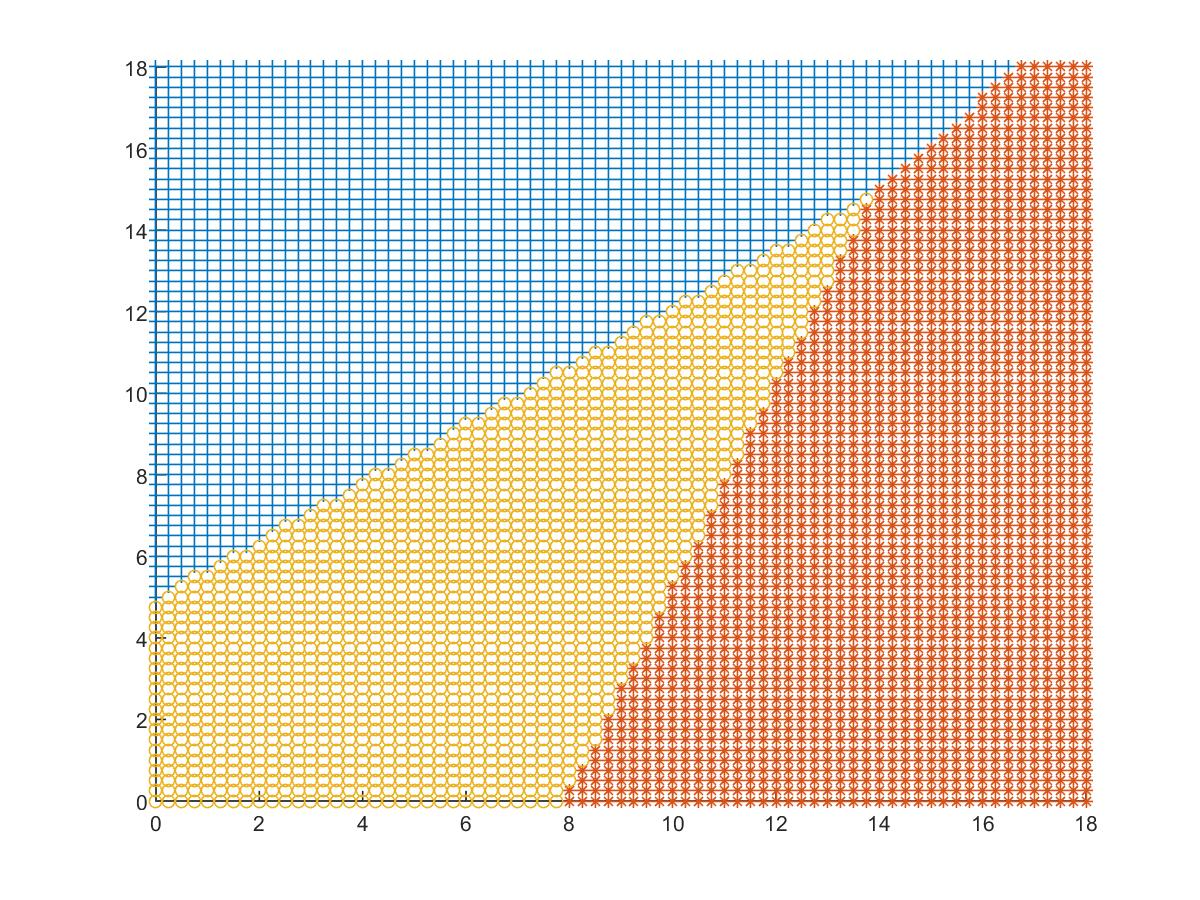
\includegraphics[height=5cm]{boundry.jpg}
\end{align*}
\end{problem}

\begin{problem}{2. Bayesian vs randomized decision}
\item{1.} Since $\alpha_{ran}$ randomly picks a class according to the posterior probabilities, we have\\ 
  $P(\alpha_{ran}(x) = i|x) = P(y=i|x)$. With 0-1 loss, we have
  \begin{align*}
	R(\alpha_{ran}) = \int_xR(\alpha_{ran}(x)|x) \cdot P(x) \cdot dx = 
	\int_x \sum_i (1-P(y=i|x)) \cdot P(y=i|x) \cdot P(x) \cdot dx
  \end{align*}
\item{2.} For Bayes decision, we have
  \begin{align*}
	& R(\alpha_{bayes}) = \int_x \sum_i (1-P(y=t|x)) \cdot P(y=i|x) \cdot P(x) \cdot dx \\
	& where\ t = argmin_j(1-P(y=j|x))
  \end{align*}
  Since $ (1-P(y=t|x)) \leq (1-P(y=j|x))$ for any x and j, we know that $R(\alpha_{ran}) \leq R(\alpha_{bayes})$
\item{3.} From b we can see that $R(\alpha_{ran}) = R(\alpha_{bayes})$ if and only if $P(y=i|x)$ are the same for all choices of i.
\end{problem}

\begin{problem}{3. ROC and PR curves}
\item{1.}
For any T, the true positive rate can be calculated by
\begin{align*}
	p(x\geq T|y=1) = 1 - normcdf(x, 9, 4^2)
\end{align*}
Similarly false positive rate is given by 
\begin{align*}
   p(x\geq T|y=-1) = 1 - normcdf(x, 3, 5^2)
\end{align*}
And false negative rate is given by
\begin{align*}
   p(x\leq T|y=1) = normcdf(x, 9, 4^2)
\end{align*}
With threashold T ranging from 20 to -10, we obtained the following curves.
\begin{align*}
& 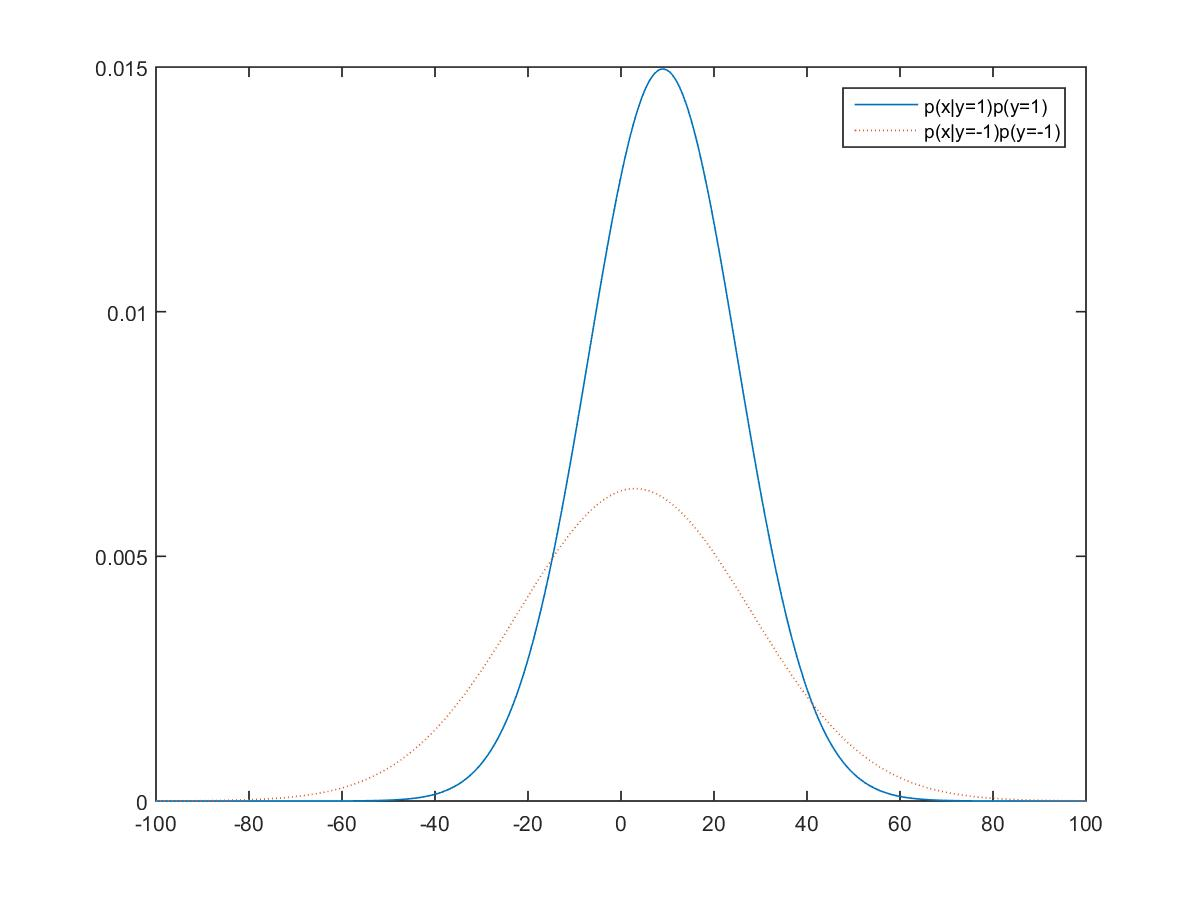
\includegraphics[height=7cm]{prob.jpg} \\
& 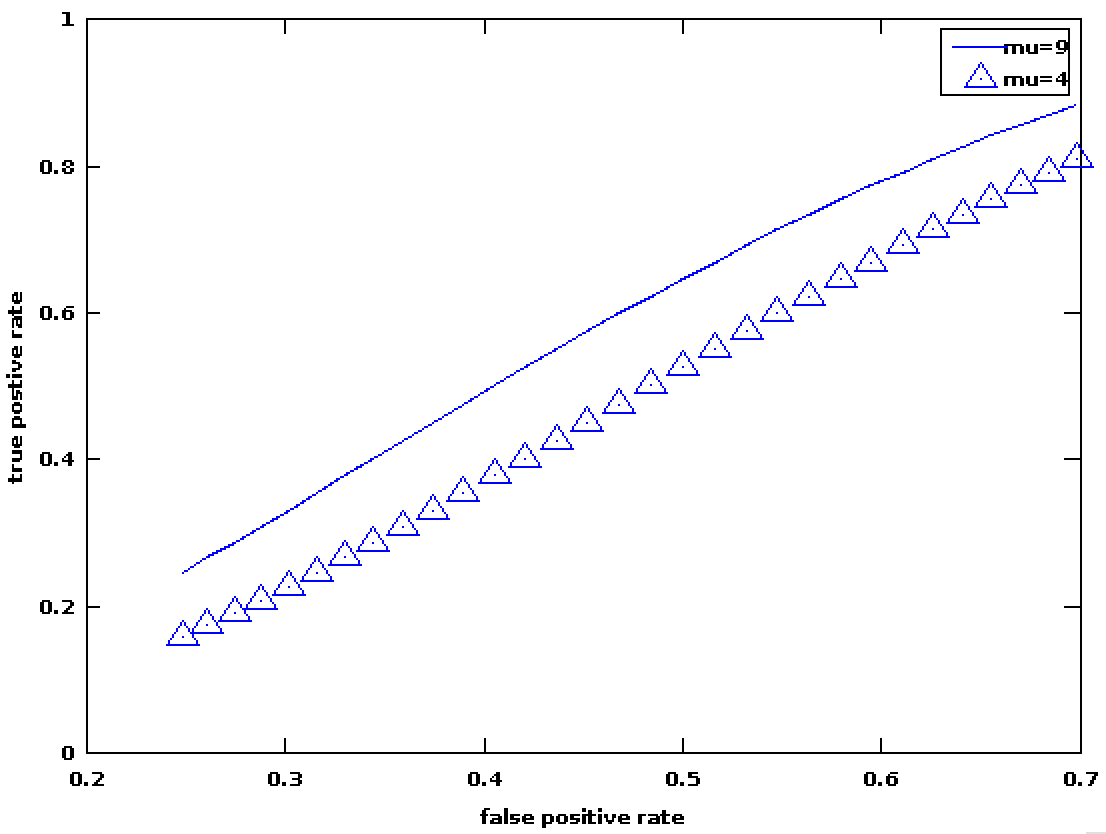
\includegraphics[height=7cm]{roc.jpg} 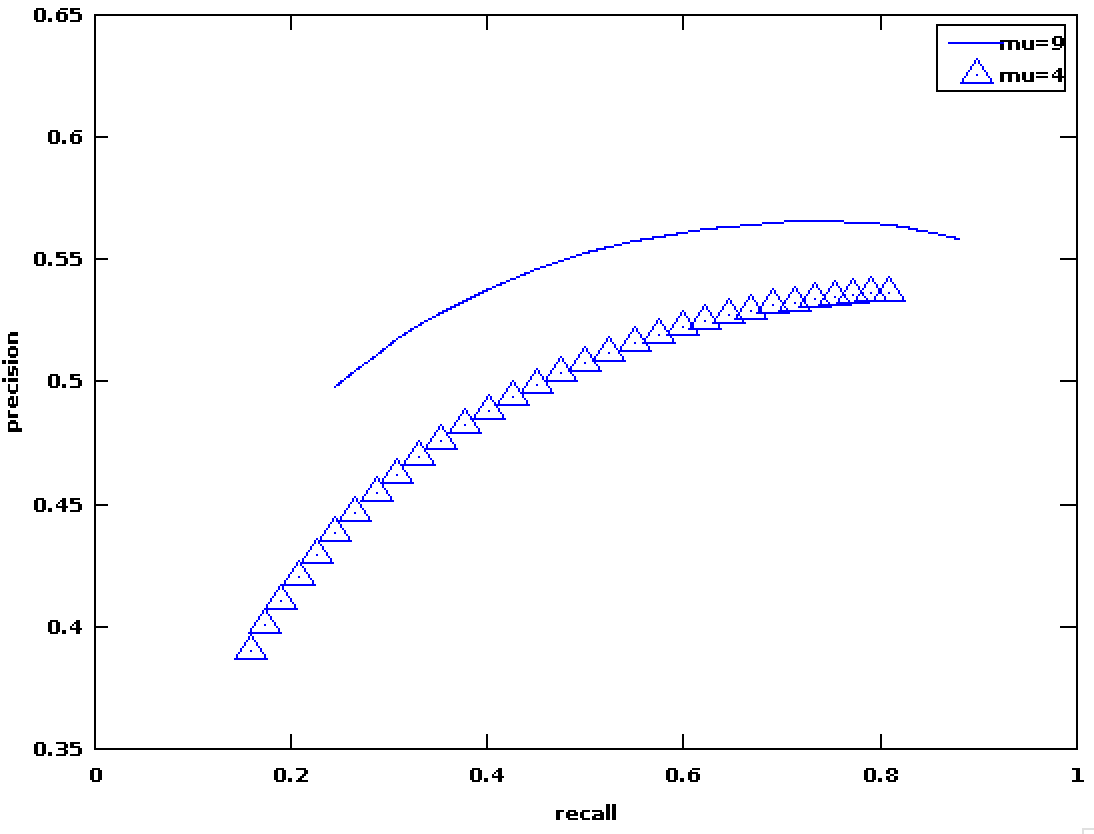
\includegraphics[height=7cm]{pr.jpg} \\
\end{align*}
\end{problem}

\begin{problem}{4. Reasoning with Bayesian rule}
\item{1.}
The outcomes of execution can be modeled by random variable X=\{1,2,3\}, indicating whether prisioner A,B or C will be executed. And the information from janitor can be represented by random variable Y=\{2,3\}, indicating the prisoner who will not be executed that A leaned from janitor.\\
The prior is thus P(X), the probability of a prisoner being executed. And the posterior is $P(X|Y)$, the probability of X being executed given Y will not be executed.
\item{2.}
	P(X) = 1/3 and the likelihood are
	\begin{align*}
	& P(Y=3|X=1) = \frac{P(X=1,Y=3)}{P(X=1)} = \frac{1}{2}\\
	& P(Y=3|X=2) = \frac{P(X=2,Y=3)}{P(Y=3)} = 1\\
	& P(Y=3|X=3) = 0\\
	\end{align*}
\item{3.} The posterior is thus
  \begin{align*}
	P(X=1|Y=3) = \frac{P(Y=3|X=1) \cdot P(X=1)}{\sum_{i=1}^{3}P(Y=3|X=i) \cdot P(X=i)} = \frac{1}{3}
  \end{align*}
\item{4.} After knowing that C is excluded, the probability of A being executed is still 1/3. So the janitor did not reveal any information about A's fate.
\end{problem}

\begin{problem}{5. Bayesian Decision}
\item The discriminant function of Bayesian decision for each actions is given by
  \begin{align*}
	g_i(\alpha(x)) = -\sum_{i=1}^{3}\lambda(\alpha (x)|y=i) \cdot P(y=i|x)
  \end{align*}
  where 
  \begin{align*}
	\lambda(\alpha(x)|y) = -
	  \begin{bmatrix}
		16000 & 16000 \\
		32000 & 8000 \\
		8000 & 32000 \\
	  \end{bmatrix}
  \end{align*}
  thus
  \begin{align*}
	& g_1(\alpha(x)) = 16000 \\
	& g_2(\alpha(x)) = 32000 \cdot 0.68 + 8000 \cdot 0.32 = 24320 \\
	& g_3(\alpha(x)) = 32000 \cdot 0.32 + 8000 \cdot 0.68 = 15680 \\
  \end{align*}
  So the Bayesian decision rule $\textit{argmax}_ig_i$ chooses $g_3$, which represents the action ''Choosing answer A''
\end{problem}

% --------------------------------------------------------------
%     You don't have to mess with anything below this line.
% --------------------------------------------------------------
 
\end{document}
